\documentclass[]{book}
\usepackage{lmodern}
\usepackage{amssymb,amsmath}
\usepackage{ifxetex,ifluatex}
\usepackage{fixltx2e} % provides \textsubscript
\ifnum 0\ifxetex 1\fi\ifluatex 1\fi=0 % if pdftex
  \usepackage[T1]{fontenc}
  \usepackage[utf8]{inputenc}
\else % if luatex or xelatex
  \ifxetex
    \usepackage{mathspec}
  \else
    \usepackage{fontspec}
  \fi
  \defaultfontfeatures{Ligatures=TeX,Scale=MatchLowercase}
  \newcommand{\euro}{€}
\fi
% use upquote if available, for straight quotes in verbatim environments
\IfFileExists{upquote.sty}{\usepackage{upquote}}{}
% use microtype if available
\IfFileExists{microtype.sty}{%
\usepackage{microtype}
\UseMicrotypeSet[protrusion]{basicmath} % disable protrusion for tt fonts
}{}
\usepackage[margin=1in]{geometry}
\usepackage{hyperref}
\PassOptionsToPackage{usenames,dvipsnames}{color} % color is loaded by hyperref
\hypersetup{unicode=true,
            pdftitle={Introdução à Análise Multivariada usando R},
            pdfauthor={Marcio Nicolau},
            pdfborder={0 0 0},
            breaklinks=true}
\urlstyle{same}  % don't use monospace font for urls
\usepackage{natbib}
\bibliographystyle{apalike}
\usepackage{color}
\usepackage{fancyvrb}
\newcommand{\VerbBar}{|}
\newcommand{\VERB}{\Verb[commandchars=\\\{\}]}
\DefineVerbatimEnvironment{Highlighting}{Verbatim}{commandchars=\\\{\}}
% Add ',fontsize=\small' for more characters per line
\usepackage{framed}
\definecolor{shadecolor}{RGB}{248,248,248}
\newenvironment{Shaded}{\begin{snugshade}}{\end{snugshade}}
\newcommand{\KeywordTok}[1]{\textcolor[rgb]{0.13,0.29,0.53}{\textbf{{#1}}}}
\newcommand{\DataTypeTok}[1]{\textcolor[rgb]{0.13,0.29,0.53}{{#1}}}
\newcommand{\DecValTok}[1]{\textcolor[rgb]{0.00,0.00,0.81}{{#1}}}
\newcommand{\BaseNTok}[1]{\textcolor[rgb]{0.00,0.00,0.81}{{#1}}}
\newcommand{\FloatTok}[1]{\textcolor[rgb]{0.00,0.00,0.81}{{#1}}}
\newcommand{\ConstantTok}[1]{\textcolor[rgb]{0.00,0.00,0.00}{{#1}}}
\newcommand{\CharTok}[1]{\textcolor[rgb]{0.31,0.60,0.02}{{#1}}}
\newcommand{\SpecialCharTok}[1]{\textcolor[rgb]{0.00,0.00,0.00}{{#1}}}
\newcommand{\StringTok}[1]{\textcolor[rgb]{0.31,0.60,0.02}{{#1}}}
\newcommand{\VerbatimStringTok}[1]{\textcolor[rgb]{0.31,0.60,0.02}{{#1}}}
\newcommand{\SpecialStringTok}[1]{\textcolor[rgb]{0.31,0.60,0.02}{{#1}}}
\newcommand{\ImportTok}[1]{{#1}}
\newcommand{\CommentTok}[1]{\textcolor[rgb]{0.56,0.35,0.01}{\textit{{#1}}}}
\newcommand{\DocumentationTok}[1]{\textcolor[rgb]{0.56,0.35,0.01}{\textbf{\textit{{#1}}}}}
\newcommand{\AnnotationTok}[1]{\textcolor[rgb]{0.56,0.35,0.01}{\textbf{\textit{{#1}}}}}
\newcommand{\CommentVarTok}[1]{\textcolor[rgb]{0.56,0.35,0.01}{\textbf{\textit{{#1}}}}}
\newcommand{\OtherTok}[1]{\textcolor[rgb]{0.56,0.35,0.01}{{#1}}}
\newcommand{\FunctionTok}[1]{\textcolor[rgb]{0.00,0.00,0.00}{{#1}}}
\newcommand{\VariableTok}[1]{\textcolor[rgb]{0.00,0.00,0.00}{{#1}}}
\newcommand{\ControlFlowTok}[1]{\textcolor[rgb]{0.13,0.29,0.53}{\textbf{{#1}}}}
\newcommand{\OperatorTok}[1]{\textcolor[rgb]{0.81,0.36,0.00}{\textbf{{#1}}}}
\newcommand{\BuiltInTok}[1]{{#1}}
\newcommand{\ExtensionTok}[1]{{#1}}
\newcommand{\PreprocessorTok}[1]{\textcolor[rgb]{0.56,0.35,0.01}{\textit{{#1}}}}
\newcommand{\AttributeTok}[1]{\textcolor[rgb]{0.77,0.63,0.00}{{#1}}}
\newcommand{\RegionMarkerTok}[1]{{#1}}
\newcommand{\InformationTok}[1]{\textcolor[rgb]{0.56,0.35,0.01}{\textbf{\textit{{#1}}}}}
\newcommand{\WarningTok}[1]{\textcolor[rgb]{0.56,0.35,0.01}{\textbf{\textit{{#1}}}}}
\newcommand{\AlertTok}[1]{\textcolor[rgb]{0.94,0.16,0.16}{{#1}}}
\newcommand{\ErrorTok}[1]{\textcolor[rgb]{0.64,0.00,0.00}{\textbf{{#1}}}}
\newcommand{\NormalTok}[1]{{#1}}
\usepackage{longtable,booktabs}
\usepackage{graphicx,grffile}
\makeatletter
\def\maxwidth{\ifdim\Gin@nat@width>\linewidth\linewidth\else\Gin@nat@width\fi}
\def\maxheight{\ifdim\Gin@nat@height>\textheight\textheight\else\Gin@nat@height\fi}
\makeatother
% Scale images if necessary, so that they will not overflow the page
% margins by default, and it is still possible to overwrite the defaults
% using explicit options in \includegraphics[width, height, ...]{}
\setkeys{Gin}{width=\maxwidth,height=\maxheight,keepaspectratio}
\setlength{\parindent}{0pt}
\setlength{\parskip}{6pt plus 2pt minus 1pt}
\setlength{\emergencystretch}{3em}  % prevent overfull lines
\providecommand{\tightlist}{%
  \setlength{\itemsep}{0pt}\setlength{\parskip}{0pt}}
\setcounter{secnumdepth}{5}

%%% Use protect on footnotes to avoid problems with footnotes in titles
\let\rmarkdownfootnote\footnote%
\def\footnote{\protect\rmarkdownfootnote}

%%% Change title format to be more compact
\usepackage{titling}

% Create subtitle command for use in maketitle
\newcommand{\subtitle}[1]{
  \posttitle{
    \begin{center}\large#1\end{center}
    }
}

\setlength{\droptitle}{-2em}
  \title{Introdução à Análise Multivariada usando R}
  \pretitle{\vspace{\droptitle}\centering\huge}
  \posttitle{\par}
  \author{Marcio Nicolau}
  \preauthor{\centering\large\emph}
  \postauthor{\par}
  \predate{\centering\large\emph}
  \postdate{\par}
  \date{2016-10-24}


% Redefines (sub)paragraphs to behave more like sections
\ifx\paragraph\undefined\else
\let\oldparagraph\paragraph
\renewcommand{\paragraph}[1]{\oldparagraph{#1}\mbox{}}
\fi
\ifx\subparagraph\undefined\else
\let\oldsubparagraph\subparagraph
\renewcommand{\subparagraph}[1]{\oldsubparagraph{#1}\mbox{}}
\fi

\usepackage{booktabs}

\begin{document}
\maketitle

{
\setcounter{tocdepth}{1}
\tableofcontents
}
\chapter{Pré-requisitos}\label{pre-requisitos}

Antes de iniciar o curso, faz-se nescessário instalar as ferramentas e
pacotes para uso.

Será utilizado o sofware \emph{R version 3.3.1 (2016-06-21)} disponível
em \href{https://cran.r-project.org}{CRAN} e o \emph{RStudio v1.0.44
Preview} disponível em
\href{https://www.rstudio.com/products/rstudio/download/preview/}{RStudio}.

A carga horária total será de 20 horas (3 dias) nos quais os seguintes
tópicos de Análise Multivariada serão abordados.

\begin{itemize}
\tightlist
\item
  Análise de Agrupamentos (CA)
\item
  Análise de Componentes Principais (PCA)
\item
  Análise Fatorial (FA)
\end{itemize}

Alguns exemplos serão realizados com dados disponíveis na literatura
científica e, em certos momentos, serão utilizados dados dos próprios
participantes.

Espera-se que ao final do curso o aluno seja capaz de entender o uso de
cada técnica e aplicá-la de forma correta em seu campo/área de pesquisa.

Cabe lembrar que este é um curso introdutório e que de forma alguma os
conteúdos e aplicações serão apresentadas de forma exaustiva.

Marcio Nicolau

Estatístico / Embrapa Trigo

Palmas/TO, Outubro de 2016

\chapter{Introdução}\label{intro}

As técnicas de Análise Multivariadas oferecem aplicações em diversas
áreas do conhecimento no desenvolvimento científico.

Geralmente são utilizadas em fase exploratória de análise de dados, onde
se busca entender melhor as relações entre as variáveis (medições
físicas ou observações) de certo evento sob estudo ou de interesse
científico.

Há também aplicações em conjunto com outros métodos da estatística onde
é possível obter validações ou testes de carácter conclusivo.

Durante este curso e, certamente limitados pelo tempo, serão abordados
somente as técnicas de caractere exploratório com a finalidade de melhor
explicar as relações intrínsecas entre os dados, reduzir a dimensão,
entender fontes de variabilidade, criar grupos homogêneos de
indivíduos/espécies.

Pode-se dizer que a Análise Fatorial (FA), a Análise de Componentes
Principais (PCA) e a Análise de Cluster (CA) são processo que tem por
objetivo reduzir a complexidade dos dados observados, bem como entender
o modelo estrutural presente nos dados.

No caso do FA, o objetivo é o de identificar construções poucos
constructos para explicar os dados observados. No caso de PCA, pode não
ser simples redução de dimensão, mas a interpretação dos componentes.

Por fim, a Análise de Cluster (CA) pode também ser usada para criar
grupos de variáveis com interesse de reduzir a complexidade dos dados
por meio da formação de grupos menores e homogêneos.

Tecnicamente, o problema de redução de dados pode ser resolvido como uma
decomposição do valor singular (SVD) da matriz original, embora a
solução mais típica seja o uso de PCA nas matrizes de covariância e/ou
correlação.

\chapter{Análise de Agrupamentos}\label{AA}

Nesta seção serão utilizados as seguinte bibliotecas do R.

\begin{Shaded}
\begin{Highlighting}[]
\NormalTok{libs <-}\StringTok{ }\KeywordTok{c}\NormalTok{(}\StringTok{'cluster'}\NormalTok{, }\StringTok{'psych'}\NormalTok{)}
\KeywordTok{sapply}\NormalTok{(libs, require, }\DataTypeTok{character.only =} \OtherTok{TRUE}\NormalTok{)}
\end{Highlighting}
\end{Shaded}

\begin{verbatim}
## Loading required package: cluster
\end{verbatim}

\begin{verbatim}
## Loading required package: psych
\end{verbatim}

\begin{verbatim}
## cluster   psych 
##    TRUE    TRUE
\end{verbatim}

\begin{Shaded}
\begin{Highlighting}[]
\NormalTok{knitr::opts_knit$}\KeywordTok{set}\NormalTok{(}\DataTypeTok{fig.width=}\DecValTok{5}\NormalTok{, }\DataTypeTok{fig.height=}\DecValTok{5}\NormalTok{, }\DataTypeTok{fig.align=}\StringTok{'center'}\NormalTok{)}
\end{Highlighting}
\end{Shaded}

\section{Processo de Agrupamento}\label{AAprocess}

Um agrupamento pode ser construído de duas formas:

\begin{itemize}
\tightlist
\item
  hierarquia: funções \emph{agnes}, \emph{diana}, \emph{mona} e
  \emph{hclust};
\item
  particionamento: funções \emph{pam}, \emph{clara}, \emph{fanny} e
  \emph{kmeans}
\end{itemize}

\section{Métodos de Agrupamento}\label{AAmethod}

Um agrupamento pode gerar os grupos utilizando algum dos métodos a
seguir (mais comuns):

\begin{itemize}
\tightlist
\item
  average: \emph{média} ou UPGMA (média dissimilaridade)
\item
  single: \emph{simple:} (vizinho mais próximo)
\item
  complete: \emph{completa} (vizinho mais distante)
\item
  ward: \emph{Ward} ou método da mínima variância.
\item
  weighted/mcquitty: \emph{média ponderada} ou WPGMA
\end{itemize}

\section{Distâncias usadas para cálculo de agrupamentos}\label{AAdist}

Para se calcular a distância entre os componentes, pode-se utilizar as
funções a seguir (mais comuns):

\begin{itemize}
\tightlist
\item
  euclidian: \emph{euclideana}, raiz da soma do quadrado das diferenças
  entre os pontos/observações (distância no plano cartesiano)
\item
  mahalanobis: \emph{Mahalanobis}, distância de cada valor em relação à
  média e covariância (também conhecida como distância estatística).
  \emph{OBS} é capaz de trabalhar a distância para observações com
  repetições. (kernel da normal multivariada)
\item
  manhattan: \emph{Manhattan}, soma das diferenças média absoluta (L1
  norm)
\item
  maximum: \emph{Máxima}, máxima distância entre dois componentes
  (supremum norm)
\item
  canberra: \emph{Canberra}, uso em valores não negativos (p.ex.
  contagem) \(\sum(|x_i - y_i| / |x_i + y_i|)\)
\item
  binary: \emph{Binária}, para valores do tipo ``on''/``off'' em que
  \(0\) representa desligado e números maiores que \(0\). A distância é
  a proporção de ``on`s''.
\item
  minkowski: \emph{Minkowski}, P-Norm ou p-ésima raíz da soma de
  potência p das diferenças.
\end{itemize}

\section{Exemplo: Força de trabalho agrícola na UE
(1993)}\label{exemplo-forca-de-trabalho-agricola-na-ue-1993}

Estes conjunto registra os dados da produção per capita e o percentual
da população que trabalha na agricultura em cada país da UE em 1993.

\begin{Shaded}
\begin{Highlighting}[]
\KeywordTok{data}\NormalTok{(agriculture)}

\NormalTok{## Calcula matriz de dissimilaridade usando distância euclidiana }
\NormalTok{## e sem padronização das variáveis}
\KeywordTok{print}\NormalTok{(}\KeywordTok{daisy}\NormalTok{(agriculture, }\DataTypeTok{metric =} \StringTok{"euclidean"}\NormalTok{, }\DataTypeTok{stand =} \OtherTok{FALSE}\NormalTok{),}
      \DataTypeTok{digits =} \DecValTok{2}\NormalTok{)}
\end{Highlighting}
\end{Shaded}

\begin{verbatim}
## Dissimilarities :
##        B   DK    D   GR    E    F  IRL    I    L   NL    P
## DK   5.4                                                  
## D    2.1  3.4                                             
## GR  22.3 22.6 22.7                                        
## E    9.8 11.2 10.4 12.6                                   
## F    3.4  3.5  2.7 20.1  8.1                              
## IRL 12.7 13.3 13.1  9.6  3.1 10.6                         
## I    5.8  5.5  5.4 17.4  5.7  2.8  7.9                    
## L    4.3  2.2  2.3 24.0 12.1  4.1 14.6  6.7               
## NL   1.6  5.1  2.4 20.8  8.3  2.2 11.2  4.2  4.7          
## P   17.2 17.9 17.7  5.2  7.4 15.2  4.6 12.5 19.2 15.7     
## UK   2.8  8.1  4.9 21.5  9.0  5.3 12.1  6.7  7.1  3.1 16.3
## 
## Metric :  euclidean 
## Number of objects : 12
\end{verbatim}

\begin{Shaded}
\begin{Highlighting}[]
\NormalTok{## Usa método de particionamento pelo meióide }
\NormalTok{## Partitioning Around Medoids (PAM)}
\KeywordTok{plot}\NormalTok{(}\KeywordTok{pam}\NormalTok{(agriculture, }\DecValTok{2}\NormalTok{), }\DataTypeTok{which.plots =} \DecValTok{1}\NormalTok{)}
\end{Highlighting}
\end{Shaded}

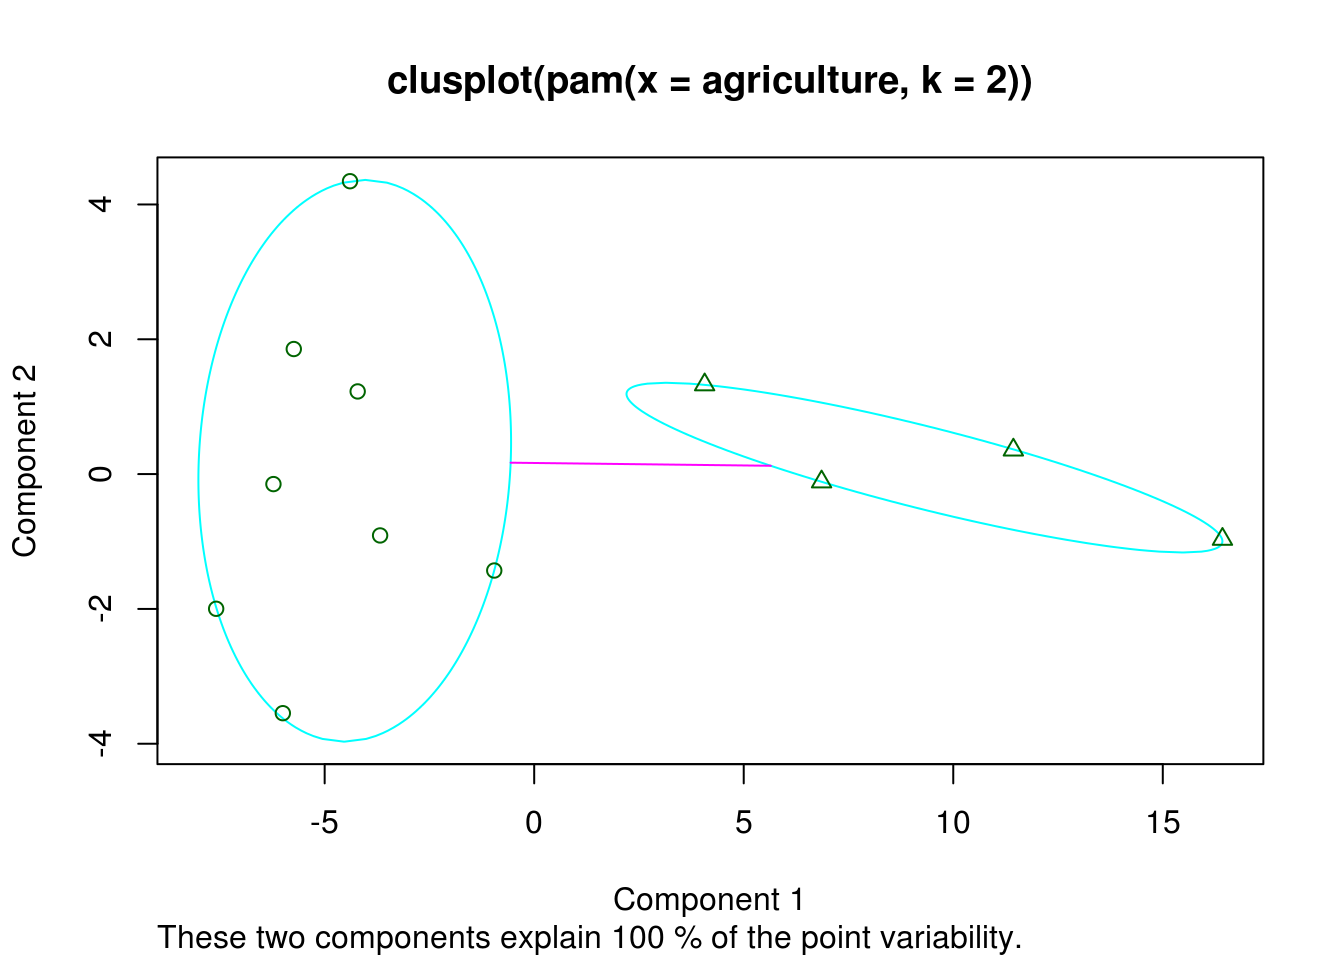
\includegraphics{r-intro-multivar_files/figure-latex/data_agri_exe-1.pdf}

\begin{Shaded}
\begin{Highlighting}[]
\NormalTok{## Gráfico dendograma usando método aglomeração mais próximo}
\NormalTok{## agnes}
\KeywordTok{plot}\NormalTok{(}\KeywordTok{agnes}\NormalTok{(agriculture), }\DataTypeTok{which.plots =} \DecValTok{2}\NormalTok{, }\DataTypeTok{hang =} \NormalTok{-}\DecValTok{1}\NormalTok{)}
\end{Highlighting}
\end{Shaded}

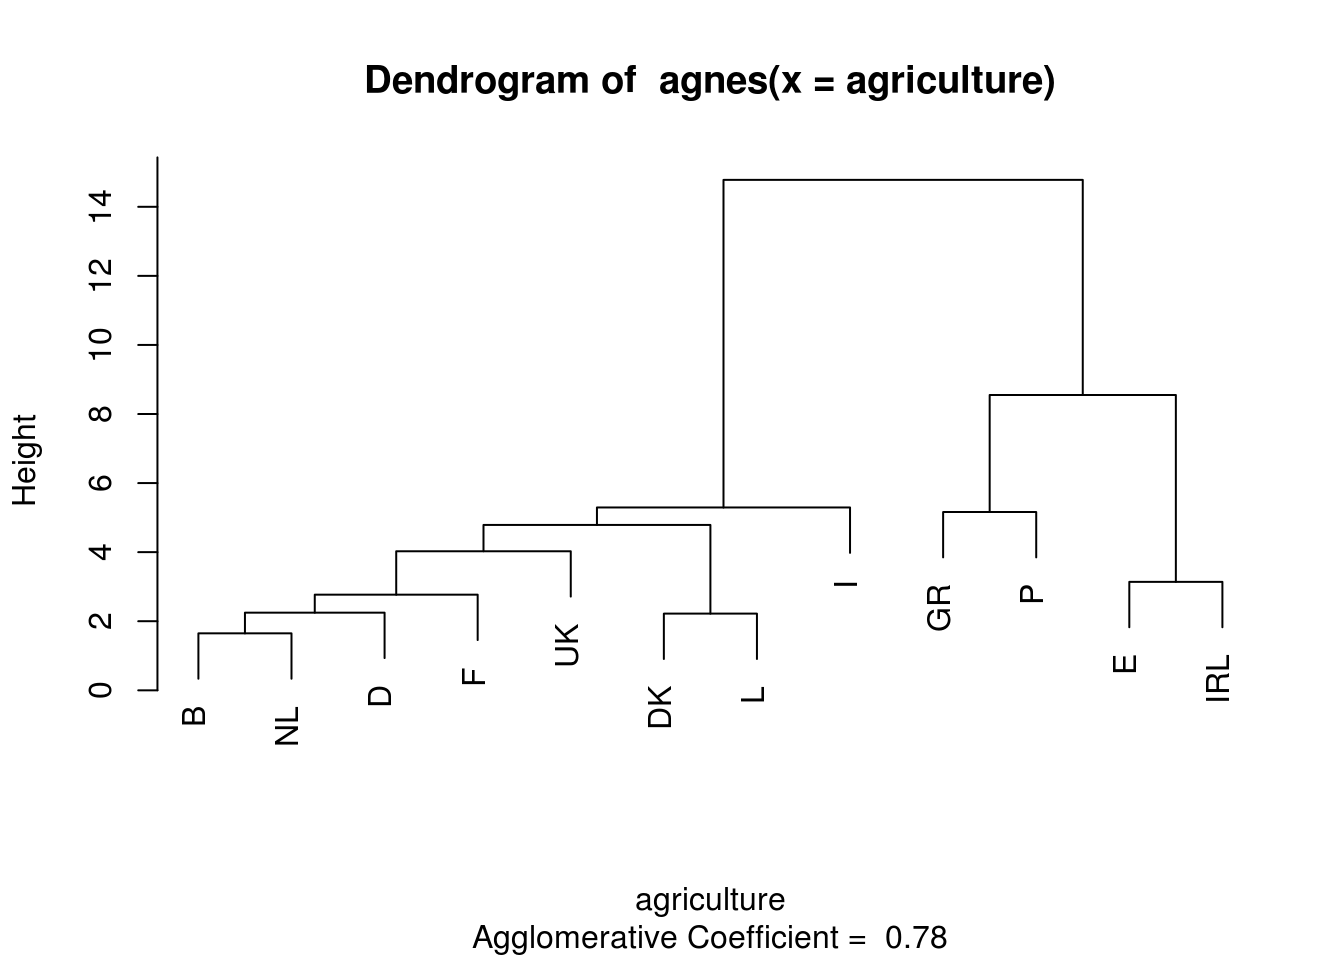
\includegraphics{r-intro-multivar_files/figure-latex/data_agri_exe-2.pdf}

\begin{Shaded}
\begin{Highlighting}[]
\NormalTok{## Plot dissimilaridade usando método divisivo}
\NormalTok{## diana}
\KeywordTok{plot}\NormalTok{(}\KeywordTok{diana}\NormalTok{(agriculture), }\DataTypeTok{which.plots =} \DecValTok{1}\NormalTok{)}
\end{Highlighting}
\end{Shaded}

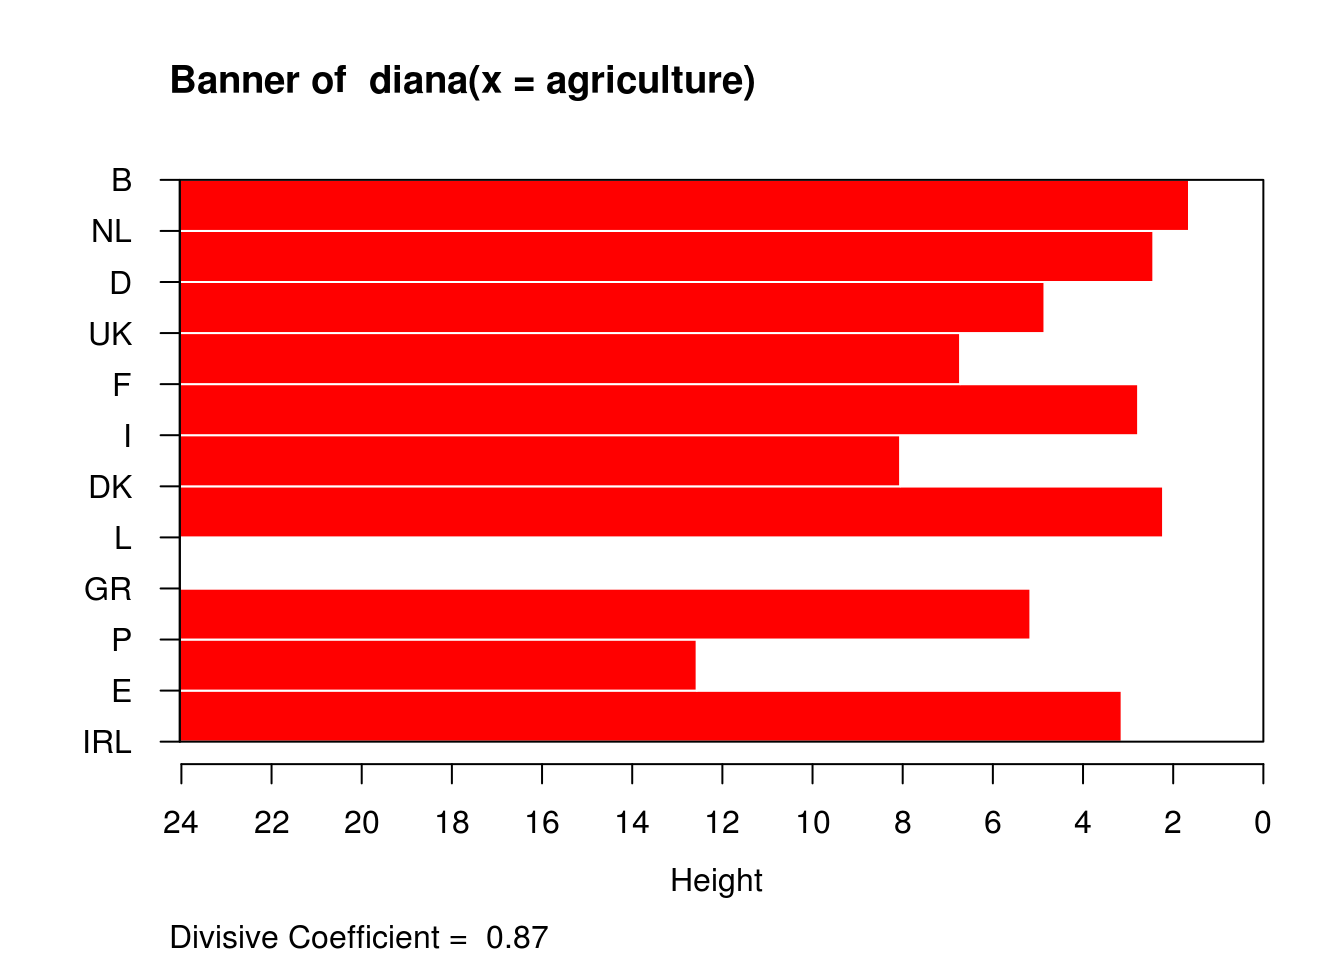
\includegraphics{r-intro-multivar_files/figure-latex/data_agri_exe-3.pdf}

\begin{Shaded}
\begin{Highlighting}[]
\NormalTok{## Usando agnes e diana para conjunto agricultura}
\KeywordTok{par}\NormalTok{(}\DataTypeTok{mfrow=}\KeywordTok{c}\NormalTok{(}\DecValTok{1}\NormalTok{,}\DecValTok{2}\NormalTok{), }\DataTypeTok{mar=}\KeywordTok{c}\NormalTok{(}\DecValTok{3}\NormalTok{,}\DecValTok{2}\NormalTok{,}\DecValTok{2}\NormalTok{,}\DecValTok{0}\NormalTok{))}
\KeywordTok{plot}\NormalTok{(}\KeywordTok{agnes}\NormalTok{(agriculture), }\DataTypeTok{which.plots =} \DecValTok{2}\NormalTok{, }\DataTypeTok{hang =} \NormalTok{-}\DecValTok{1}\NormalTok{,}
     \DataTypeTok{main =} \StringTok{"Método Aglomerativo}\CharTok{\textbackslash{}n}\StringTok{AGNES"}\NormalTok{)}
\KeywordTok{plot}\NormalTok{(}\KeywordTok{diana}\NormalTok{(agriculture), }\DataTypeTok{which.plots =} \DecValTok{2}\NormalTok{, }\DataTypeTok{hang =} \NormalTok{-}\DecValTok{1}\NormalTok{,}
     \DataTypeTok{main =} \StringTok{"Método Divisivo}\CharTok{\textbackslash{}n}\StringTok{DIANA"}\NormalTok{)}
\end{Highlighting}
\end{Shaded}

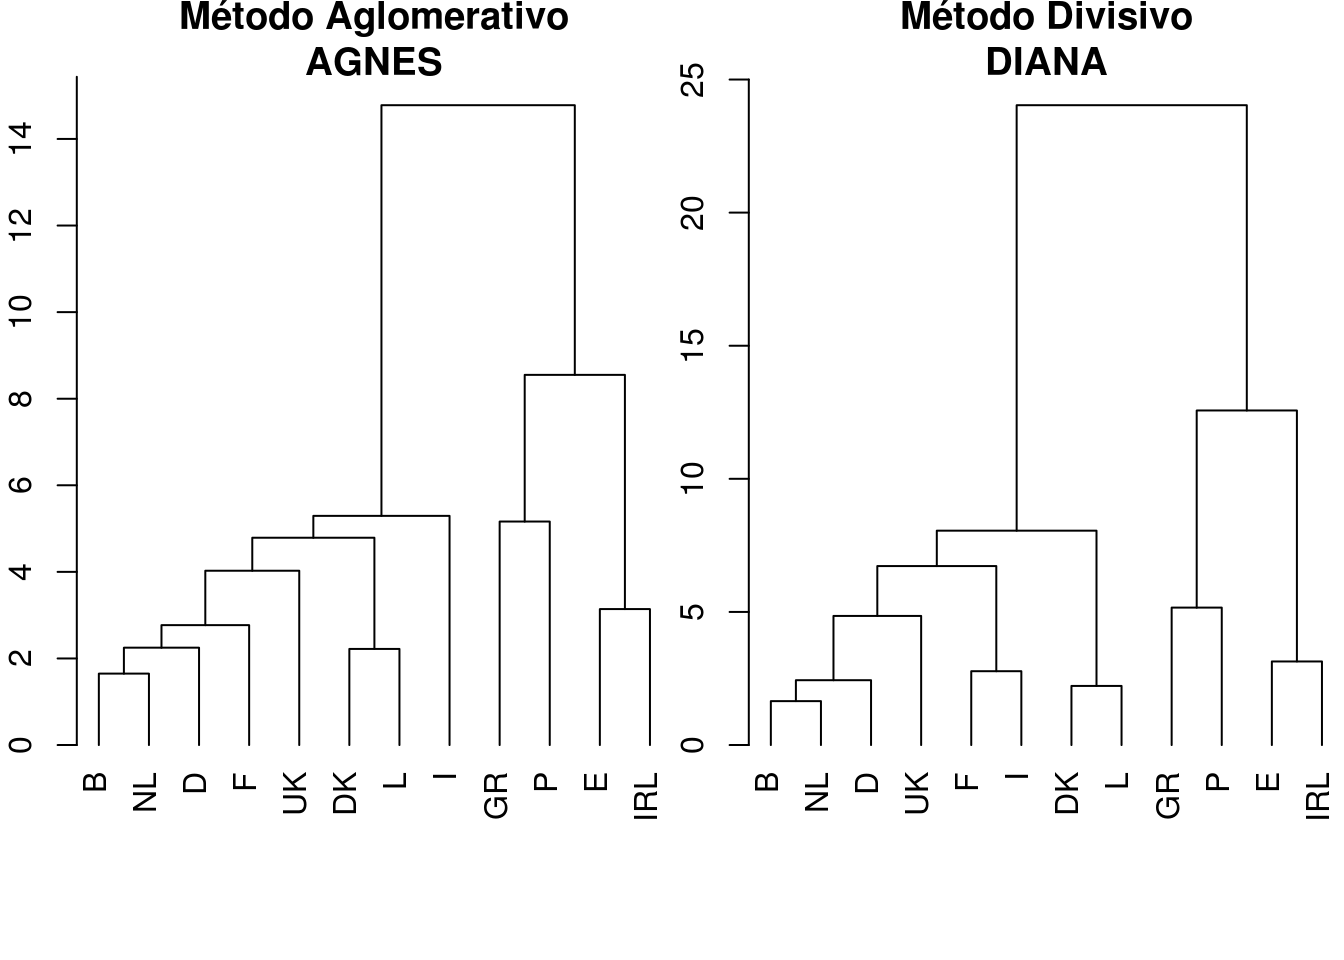
\includegraphics{r-intro-multivar_files/figure-latex/data_agri_exe-4.pdf}

\begin{Shaded}
\begin{Highlighting}[]
\KeywordTok{par}\NormalTok{(}\DataTypeTok{mfrow=}\KeywordTok{c}\NormalTok{(}\DecValTok{1}\NormalTok{,}\DecValTok{1}\NormalTok{))}
\end{Highlighting}
\end{Shaded}

\chapter{Análise de Componentes Principais}\label{PCA}

É uma alternativa à Análise Fatorial (FA), apesar dos objetivos serem
semelhantes (PCA e FA), na PCA se busca obter o modelo descritivo dos
dados enquanto na FA se busca o modelo estrutural.

Outro destaque importante é que a matriz/vetor de cargas
\emph{``loadings''} possuírem valores equivalentes, na FA estes são
menores. Isto ocorre porque na PCA é ajustado um modelo para a variância
completa da matriz de correlação das variáveis e na FA o processo é
realizado somente para a variância comum.

\chapter{Análise Fatorial}\label{FA}

Some \emph{significant} applications are demonstrated in this chapter.

\section{Example one}\label{example-one}

\section{Example two}\label{example-two}

\bibliography{packages.bib,book.bib}

\end{document}
